\begin{multicols}{2}
\CKEcontents{}{}

\section{Hamility}

  Laele~\cite{ctn:FR1}, Final list. Another example of citation: Laele~\upcite{ctn:FR1}.

  \lipsum[1-2]
  
  \begin{question}[Uncountable Monkeys]
    \lipsum[5]
  \end{question}

  \url{https://www.google.com}

\section{Honor}
  \lipsum[3]

\section{Scarifice}
  \lipsum[4]

\renewsecnum{9}
\renewfignum{2}
\begin{figure*}
  \centering
  \subfloat[Two complementary functions.]{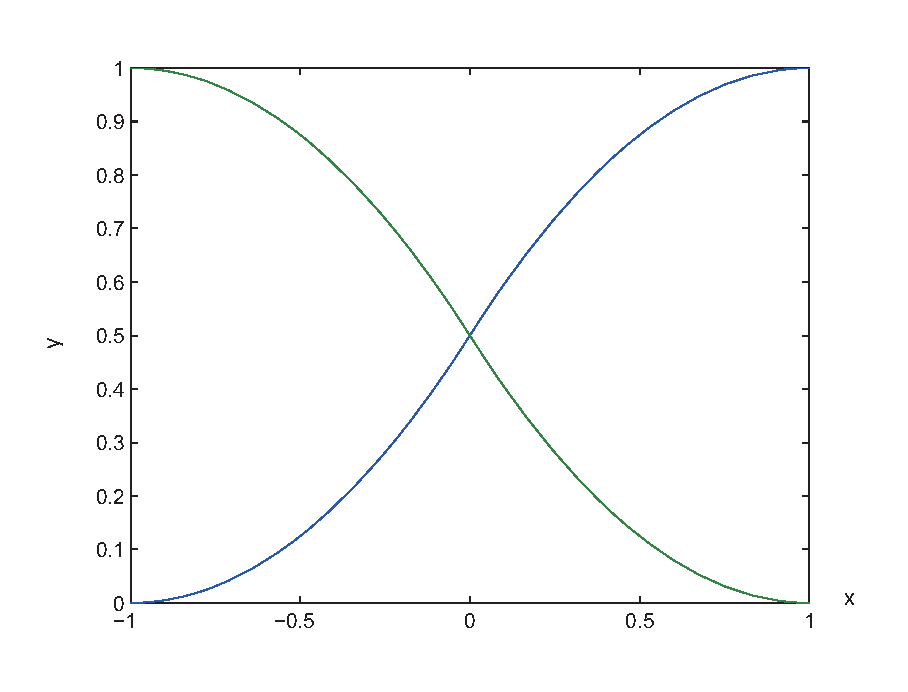
\includegraphics[width=0.8\columnwidth]{test1}}
  \subfloat[A wave with envelop2.]{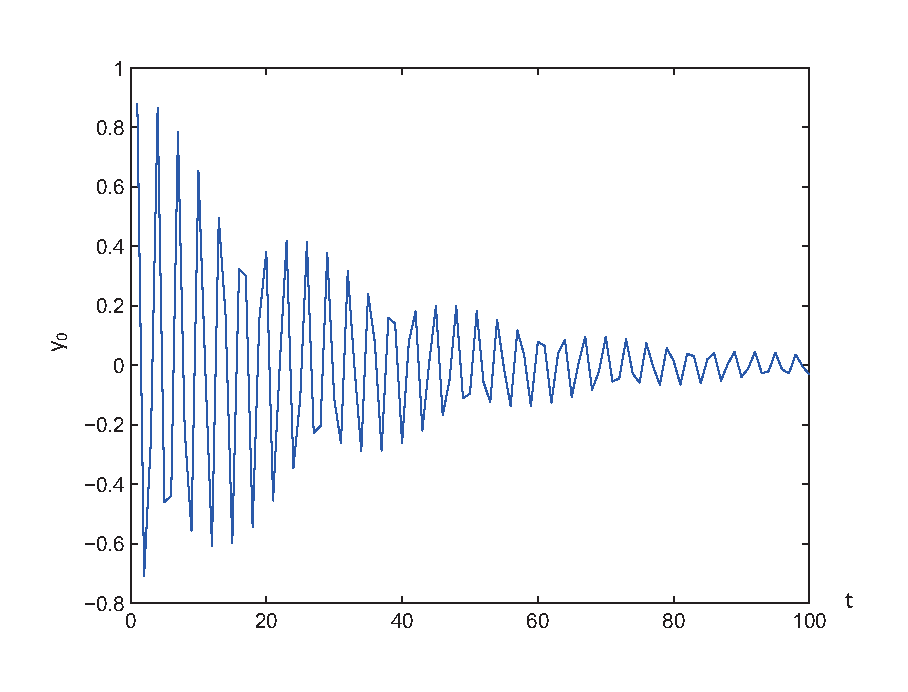
\includegraphics[width=0.8\columnwidth]{test2}}
  \DeclareGraphicsExtensions.
  \caption{Test graphs.} \label{fig:test}
\end{figure*}
\renewsecnum{3}
\renewfignum{1}

\section{Valor}
  \lipsum[6]

\section{Compassion}
  \lipsum[7-9]

\section{Spirituality}
  \lipsum[10]

\section{Honesty}
  \lipsum[11]

\section{Justice}
  \lipsum[12]

\section{Enhancements}

\subsection{Special table}

\autoref{tab:bdbasd} is an example of the table in this class. We use \texttt{$\backslash$hlinerev} to switch the color of the next row. When the argument is 1, the next row would be colored by gray. If use 0, the next row would be colored by white. \texttt{$\backslash$hlinedge} is used for setting thickness of the first and the bottom line.

\begin{table}[H]
  \centering
  \vspace{-1.5em}
  \caption{Module Test} \label{tab:bdbasd}
  \begin{tabular}{m{0.2\columnwidth}m{0.27\columnwidth}m{0.27\columnwidth}}
    \hlinedge{1.2pt}
    % after \\: \hline or \cline{col1-col2} \cline{col3-col4} ...
    \multirow{2}{*}{Data} & \multicolumn{2}{c}{Result}  \\ \cline{2-3}
    & Normal & Reverse  \\ \hline
    Min Loss [dB]  & -4.1005 &  -4.1081  \hlinerev{1}
    Max Loss [dB] & -50.6748 & -50.3463  \hlinerev{0}
    BDwidth [MHz] & 394.5 & 394.5  \\ \hlinedge{1.2pt}
  \end{tabular}
\end{table}

\subsection{Subfigures}

First, we show a regular figure in \autoref{fig:testreg}.

\begin{figure}[H]
  \centering
  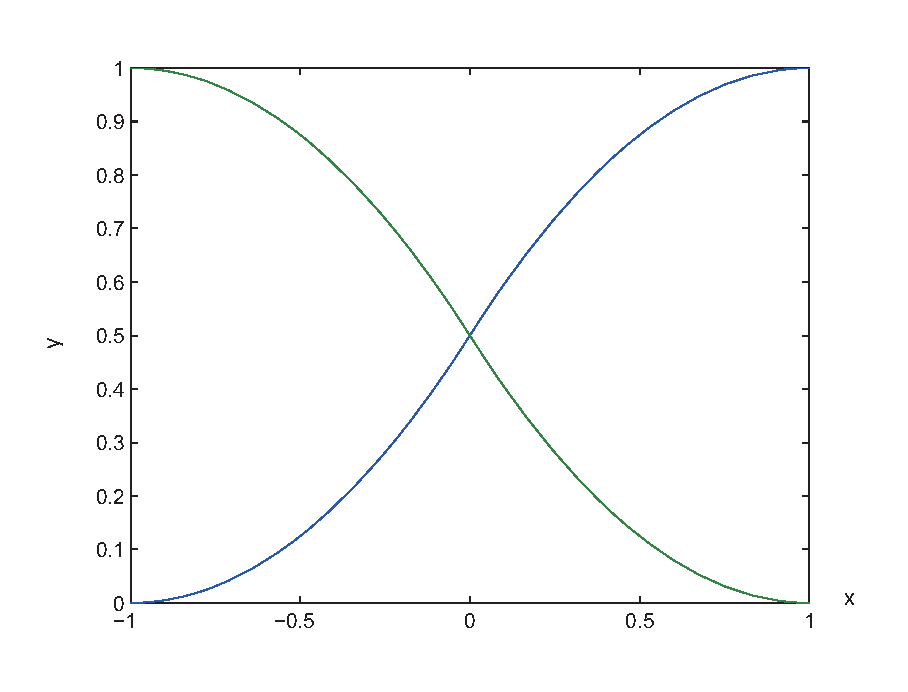
\includegraphics[width=0.8\columnwidth]{test1}
  \DeclareGraphicsExtensions.
  \caption{A regular example of the figure.} \label{fig:testreg}
\end{figure}

In \autoref{fig:test} we show an example of a figure crossing two columns and containing 2 subfigures. This feature is supported by \texttt{stfloats} and \texttt{subfig}. To place this figure in the correct position, we may need to adjust the place of the figure manually, which may cause a wrong caption number. To fix this problem, we provide the following command for changing the current counter:

\begin{lstlisting}[language=tex]
\renewsecnum{number} % Set the section number.
\renewtabnum{number} % Set the table number.
\renewfignum{number} % Set the figure number.
\reneweqnum{number}  % Set the equation number.
\end{lstlisting}

However, change the figure position may violate the order in the list of figures. Users need to pay attention to this problem.

\subsection{Algorithm}

Test Algorithm in \autoref{alg:Algorithm}:

\begin{algorithm}[H]
  \caption{DWT Algorithm}
  \label{alg:Algorithm}
  \begin{algorithmic}[1]
    \REQUIRE Sequence $\mathbf{x}$ in time domain
    \ENSURE Sequence $\hat{\mathbf{x}}$ in wavelet domain
    % if-then-else
    \STATE N = $\left\lfloor \log_2 (\mathrm{length}(\mathbf{x})) \right\rfloor$;
    \STATE $\mathbf{c}_{N} = \mathbf{x},~ \hat{\mathbf{x}} = \varnothing$;
    \FOR{$i$ from $1$ to $N$}
    \STATE $\mathbf{c}_{N-i},~\mathbf{d}_{N-i}~=~\mathrm{analysis\_filter}(\mathbf{c}_{N-i+1})$;
    \STATE insert $\mathbf{d}_{N-i}$ at the beginning of $\hat{\mathbf{x}}$.
    \ENDFOR
  \end{algorithmic}
\end{algorithm}

\subsection{Shaded quote}

We provide a style for quotation. To make use of it, call the \texttt{shadedQuote} environment.

\begin{shadeQuote}{}
  This sentence is written by an unknown person.
\end{shadeQuote}

\begin{shadeQuote}{Shakespeare}
  To be or not to be, that is the question.
\end{shadeQuote}

\begin{shadeQuote}[r]{Shakespeare}
  To be or not to be, that is the question.
\end{shadeQuote}

\subsection{Signature}

User could insert a signature by using the environment \texttt{signature}. An example is shown as follows:

\begin{signature}{0.9\columnwidth}{0.8in}{12em}{Sign.eps}
  \textbf{Name:} Yuchen Jin \\
  \textbf{Organization:} University of Houston \\
  \textbf{E-mail:} cainmagi@gmail.com \\
  \textbf{Tel:} XXX-XXX-XXXX \\
\end{signature}

The environment has 4 arguments, they are

\begin{enumerate}[(1)]
  \item The width of the whole signature.
  \item The width of the figure.
  \item The width of the descriptions.
  \item The path of the figure.
\end{enumerate}

User could also change the definition of \texttt{$\backslash$InnerSignature}, this signature would appear in the front page if the option \texttt{$\backslash$innerSig} is enabled.

\subsection{Front page and contents}

We use the following command to add a front page.
\begin{lstlisting}[language=tex]
\titlepage{1} % Could be 1 or 2
\end{lstlisting}
where the argument is the style. Could be 1 or 2.

The contents is dumped by \texttt{$\backslash$CKEcontents}. The first argument is the type of the content, the second argument is the text of the contents title. If the second argument is left blank, would generate the title automatically. Here we show some examples:
\begin{lstlisting}[language=tex]
\CKEcontents{}{} % The contents for the whole report.
\CKEcontents{tab}{} % List of tables
\CKEcontents{fig}{} % List of figures
\CKEcontents{theorem}{} % List of theorems
\end{lstlisting}

We also provide an optional argument, to enable users to insert the two-column list in the one-column text. Use a command like this:
\begin{lstlisting}[language=tex]
\CKEcontents[2col]{}{}
\end{lstlisting}

\subsection{Import files}

Basically, \LaTeX provide a method for import other \texttt{.tex} files:
\begin{lstlisting}[language=tex]
\include{example.tex}
\end{lstlisting}

We define an enhanced version, like this
\begin{lstlisting}[language=tex]
\import{example.tex}
\end{lstlisting}

This command would search the folder \texttt{./Documents} and include the file. Before including the file, all counters would be reset by 0.

To import \texttt{.pdf} files, use the following command:
\begin{lstlisting}[language=tex]
\includepage{1-2}{example.pdf}
\end{lstlisting}

The first argument is the pages that would be included, the second argument is the path of the pdf.

If users want to include a pdf file and insert it in the title, we could use
\begin{lstlisting}[language=tex]
\includepagetoc{1-2}{example.pdf}{Example PDf}
\end{lstlisting}

The third argument would be added into the contents. It would be included as a section.

This function is supported by \texttt{pdfpages} package.

\subsection{Encryption}

If users set the \texttt{ownerpass} and \texttt{userpass} (optional) by \texttt{$\backslash$ckesetup}, and compile the report by \XeLaTeX, the report would be protected by the passwords. This feature does not work with pdf\LaTeX.

\subsection{Other options}

The detail usage of the options could be referred in the readme file. In \autoref{tab:options} we only introduce some important features:

\begin{table}[H]
  \centering
  \vspace{-1.5em}
  \caption{List of options} \label{tab:options}
  \begin{tabular}{>{\small\ttfamily}m{0.24\columnwidth}m{0.6\columnwidth}}
    \hlinedge{1.2pt}
    % after \\: \hline or \cline{col1-col2} \cline{col3-col4} ...
    \textbf{\textrm{\normalsize Option}} & \textbf{Description} \\ \hline
    linkColor & Make all links colored. \hlinerev{1}
    innerSig & Add a signature in the front page. \hlinerev{0}
    refNum & Add a section number to the reference. \hlinerev{1}
    CSensLabel & Make all captions start with a section number. \\ \hlinedge{1.2pt}
  \end{tabular}
\end{table}

\bibliographystyle{IEEEtran}
% argument is your BibTeX string definitions and bibliography database(s)
\bibliography{IEEEabrv,bib/ref}

\end{multicols}

%----------------------------------------------------------------------------------------
%	Appendix
%----------------------------------------------------------------------------------------
\section*{Appendix}

\begin{appendix}

  \lipsum[13]

  \begin{enumerate}
    \item AAA
    \item BBB
    \item Caption
    \item Finally $\cdots$
  \end{enumerate}

\end{appendix}

\includepage{1}{pdfs/test.pdf}

\CKEcontents{tab}{}

\CKEcontents{fig}{}

\CKEcontents{question}{List of Questions}

%---------------------------------------------------------------------------------------- 